\documentclass{../../../oss-classkick}
\usepackage{amssymb}
\usepackage{bm}

\begin{document}
\genheader

\gentitle{C}{DYNAMICS}

\genmultidirections

\gengravity

\raggedcolumns
\begin{multicols*}{2}
  \begin{enumerate}[leftmargin=18pt]
  \item A small moving block collides with a large block at rest. Which of the
    following is true of the forces the blocks apply to each other
    \begin{enumerate}[noitemsep,topsep=0pt,leftmargin=18pt,label=(\Alph*)]
    \item The small block exerts twice the force on the large block
      compared to the force the large block exerts on the small block.
    \item The small block exerts half the force on the large block compared
      to the force the large block exerts on the small block.
    \item The small block exerts exactly the same amount of force on the
      large block that the large block exerts on the small block.
    \item The large block exerts a force on the small block, but the small
      block does not exert a force on the large block.
    \item The small block exerts a force on the large block, but the large
      block does not exert a force on the small block.
    \end{enumerate}
    \vspace{.6in}
  \end{enumerate}
  
  \textbf{Questions \ref{q:2blocks1}--\ref{q:2blocks2}}

  Two blocks, 4 kg and 2 kg, are connected by a string. An applied force $F$ of
  magnitude 18 N pulls the blocks to the left.
  \begin{center}
    \begin{tikzpicture}[scale=.95]
      \fill[pattern=north east lines] (2.5,0) rectangle(9,-.3);
      \begin{scope}[thick]
        \draw (2.5,0)--(9,0);
        \draw (7,0) rectangle(8,1) node[midway]{2 kg};
        \draw (4,0) rectangle(6,1) node[midway]{4 kg};
        \draw (6,.5)--(7,.5);
        \draw[->] (4,.5)--(3,.5) node[midway,above]{\SI{18}{\newton}};
      \end{scope}
    \end{tikzpicture}
  \end{center}
  \begin{enumerate}[resume,leftmargin=18pt]    
  \item The acceleration of the 4-kg block is
    \begin{enumerate}[nosep,leftmargin=18pt,label=(\Alph*)]
    \item\SI2{\metre\per\second\squared}
    \item\SI3{\metre\per\second\squared}
    \item\SI4{\metre\per\second\squared}
    \item\SI{4.5}{\metre\per\second\squared}
    \item\SI6{\metre\per\second\squared}
    \end{enumerate}
    \label{q:2blocks1}
    
  \item The tension in the string between the blocks is
    \begin{enumerate}[noitemsep,topsep=0pt,leftmargin=18pt,label=(\Alph*)]
    \item 4 N
    \item 6 N
    \item 12 N
    \item 16 N
    \item 18 N
    \end{enumerate}
    \label{q:2blocks2}
  \end{enumerate}

  \textbf{Questions \ref{q:striaght1}--\ref{q:striaght2}}

  An object of mass $m$ moves along a straight line with a speed described by
  the equation $v=c+bt^3$.
  \begin{enumerate}[resume,leftmargin=18pt]
  \item The initial velocity of the mass is
    \begin{enumerate}[nosep,leftmargin=18pt,label=(\Alph*)]
    \item $c$
    \item $ct+bt^3$
    \item $ct+bt^4$
    \item $bt^2$
    \item $bt$
    \end{enumerate}
    \label{q:striaght1}

  \item The net force acting on the mass at time $T$ is
    \begin{enumerate}[nosep,leftmargin=18pt,label=(\Alph*)]
    \item $3mbT$
    \item $3mbT^2$
    \item $3mbT^3$
    \item $mc+2mbT^2$
    \item $mc^2+4mbT^4$
    \end{enumerate}
    \label{q:striaght2}
    \vspace{.7in}
  \end{enumerate}  
  \columnbreak
  
  \textbf{Questions \ref{q:pulley1}--\ref{q:pulley2}}

  A system consists of two blocks having masses of \SI{2}{\kilo\gram} and
  \SI{1}{\kilo\gram}. The blocks are connected by a string of negligible mass
  and hung over a light pulley, and then released from rest.
  \begin{center}
    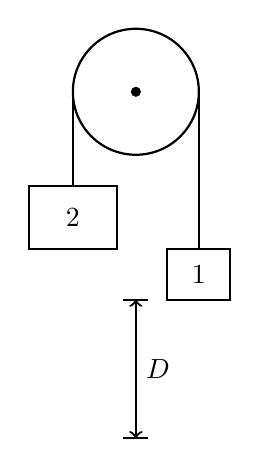
\begin{tikzpicture}[scale=.8]
      \begin{scope}[thick]
        \draw(0,0) circle(1);
        \fill(0,0) circle(.08);
        \draw(1,0)--(1,-2.5);
        \draw(.5,-2.5) rectangle(1.5,-3.3) node[midway]{\SI1{\kilo\gram}};
        \draw(-1,0)--(-1,-1.5);
        \draw(-1.7,-1.5) rectangle(-.3,-2.5) node[midway]{\SI2{\kilo\gram}};
        \draw(-.2,-3.3)--(.2,-3.3);
        \draw(-.2,-5.5)--(.2,-5.5);
        \draw[<->](0,-3.3)--(0,-5.5) node[midway,right]{$D$};
      \end{scope}
    \end{tikzpicture}
  \end{center}
  \begin{enumerate}[resume,leftmargin=18pt]
  \item The acceleration of the \SI{2}{\kilo\gram} block is most nearly
    \begin{enumerate}[nosep,leftmargin=18pt,label=(\Alph*)]
    \item $\displaystyle\frac{2}{9}g$
    \item $\displaystyle\frac{1}{3}g$
    \item $\displaystyle\frac{1}{2}g$
    \item $\displaystyle\frac{2}{3}g$
    \item $g$
    \end{enumerate}
    \label{q:pulley1}
    
  \item The speed of the \SI{2}{\kilo\gram} block after it has descended a
    distance $D$ is most nearly
    \begin{enumerate}[nosep,leftmargin=18pt,label=(\Alph*)]
    \item $\displaystyle\sqrt{\frac{4gD}{3}}$
    \item $\displaystyle\sqrt{\frac{2gD}{3}}$
    \item $\displaystyle\sqrt{\frac{gD}{3}}$
    \item $\displaystyle\sqrt{\frac{gD}{2}}$
    \item $\displaystyle\sqrt{\frac{4gD}{6}}$
    \end{enumerate}
    \label{q:pulley2}
  \end{enumerate}
  
  \textbf{Questions \ref{q:2cords1}--\ref{q:2cords2}}

  A weight of magnitude $W$ is suspended in equilibrium by two cords, one
  horizontal and one slanted at an angle of \ang{60} from the horizontal, as
  shown.
  \begin{center}
    \begin{tikzpicture}[scale=.85]
      \fill[pattern=north east lines] (0,0)--(5,0)--(5,.2)--(-.2,.2)--
      (-.2,-3)--(0,-3)--cycle;
      \begin{scope}[thick]
        \draw (0,-3)--(0,0)--(5,0);
        \draw (0,-1.5)--(1.5,-1.5)--(1.5,-2.5);
        \draw[dashed](1.5,0)--(1.5,-1.5)--(5,-1.5);
        \fill(1.5,-1.5) circle(.1);
        \draw(1.25,-2.5) rectangle(1.75,-3) node[midway]{$W$};
        \draw(1.5,-1.5)--(4.5,0);
        \draw[<->](3,-1.5) arc(0:27:1.5) node[midway,right]{\ang{60}};
      \end{scope}
    \end{tikzpicture}
  \end{center}
  \begin{enumerate}[resume,leftmargin=18pt]
  \item Which of the following statements is true?
    \begin{enumerate}[nosep,leftmargin=18pt,label=(\Alph*)]
    \item The tension in the horizontal cord must be greater than the tension
      in the slanted cord.
    \item The tension in the slanted cord must be greater than the tension in
      the horizontal cord.
    \item The tension is the same in both cords.
    \item The tension in the horizontal cord equals the weight $W$.
    \item The tension in the slanted cord equals the weight $W$.
    \end{enumerate}
    \label{q:2cords1}
    \vspace{.7in}
    
  \item The tension in the horizontal cord is
    \begin{enumerate}[nosep,leftmargin=18pt,label=(\Alph*)]
    \item equal to the tension in the slanted cord
    \item one-third as much as the tension in the slanted cord
    \item one-half as much as the tension in the slanted cord
    \item twice as much as the tension in the slanted cord
    \item three times as much as the tension in the slanted cord
    \end{enumerate}
    \label{q:2cords2}
  \end{enumerate}
  \columnbreak
  
%  \item A wooden block slides down a frictionless inclined plane a distance of
%    $1$ meter along the plane during the first second. The distance traveled
%    along the plane by the block during the time between \SI{1}{s} and \SI{2}{s}
%    is
%    \begin{enumerate}[noitemsep,topsep=0pt,leftmargin=18pt,label=(\Alph*)]
%    \item\SI{2}{\metre}
%    \item\SI{3}{\metre}
%    \item\SI{4}{\metre}
%    \item\SI{6}{\metre}
%    \item\SI{8}{\metre}
%    \end{enumerate}

  %\item A mass located at point $P$ follows a parabolic path. Which of the
  %  following diagrams indicates a possible combination of the net force $F$
  %  acting on the mass, the velocity $v$, and acceleration $a$ of the mass at
  %  point $P$?
  %  \begin{enumerate}[noitemsep,topsep=0pt,leftmargin=18pt,label=(\Alph*)]
  %  \item
  %  \item
  %  \item
  %  \item
  %  \item
  %  \end{enumerate}
  
  \textbf{Questions \ref{3blks1}--\ref{3blks2}}

  Three blocks of mass \SI{3}{\kilo\gram}, \SI{2}{\kilo\gram}, and
  \SI{1}{\kilo\gram} are pushed along a horizontal frictionless plane by a
  force of \SI{24}{\newton} to the right, as shown.
  \begin{center}
    \begin{tikzpicture}[scale=.9]
      \fill[pattern=north east lines] (0,0) rectangle(8,-.3);
      \begin{scope}[thick]
        \draw (0,0)--(8,0);
        \draw (2,0) rectangle(4,1.5) node[midway]{3 kg};
        \draw (4,0) rectangle(5.5,1.3) node[midway]{2 kg};
        \draw (5.5,0) rectangle(6.5,1.1) node[midway]{1 kg};
        \draw[->](0,.75)--(2,.75) node[midway,above]{24 N};
      \end{scope}
    \end{tikzpicture}
  \end{center}
  \begin{enumerate}[resume,leftmargin=18pt]
  \item The acceleration of the \SI{2}{\kilo\gram} block is
    \begin{enumerate}[nosep,leftmargin=18pt,label=(\Alph*)]
    \item\SI{144}{\metre\per\second\squared}
    \item\SI{72}{\metre\per\second\squared}
    \item\SI{12}{\metre\per\second\squared}
    \item\SI{6}{\metre\per\second\squared}
    \item\SI{4}{\metre\per\second\squared}
    \end{enumerate}
    \label{3blks1}
    
  \item The force that the \SI{2}{\kilo\gram} block exerts on the
    \SI{1}{\kilo\gram} block is
    \begin{enumerate}[nosep,leftmargin=18pt,label=(\Alph*)]
    \item \SI{2}{\newton}
    \item \SI{4}{\newton}
    \item \SI{6}{\newton}
    \item \SI{24}{\newton}
    \item \SI{144}{\newton}
    \end{enumerate}
    \label{3blks2}
    
%  \item A hockey puck slides along horizontal ice with a velocity $\mb{v}_1$
%    when it is struck by a hockey stick, changing its direction, as shown.
%    After the puck is struck, it has a velocity $\mb{v}_2$, which is greater
%    than $\mb{v}_1$. Which of the following vectors best represents the
%    direction the force of the hockey stick acted on the puck?
%    \begin{center}
%      \begin{tikzpicture}[scale=.6]
%        \draw[ultra thick,->](0,0)--(2,0) node[midway,below]{$\mb{v}_1$};
%        \draw[ultra thick,->](4,0)--(4,2.5) node[midway,right]{$\mb{v}_2$};
%        \draw[dashed](0,0)--(4,0)--(4,3.5);
%      \end{tikzpicture}
%    \end{center}
%    \begin{enumerate}[noitemsep,topsep=0pt,leftmargin=18pt,label=(\Alph*)]
%    \item$\uparrow$
%    \item$\leftarrow$
%    \item$\rightarrow$
%    \item$\nwarrow$
%    \item$\nearrow$
%    \end{enumerate}
    
  \item A block of mass \SI{4}{\kilo\gram} slides down a rough incline with a
    constant speed. The angle the incline makes with the horizontal is
    \ang{30}. The coefficient of friction acting between the block and incline
    is most nearly
    \begin{center}
      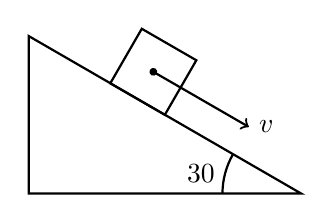
\begin{tikzpicture}
        \begin{scope}[thick]
          \draw(0,0)--(-3.46,0)--(-3.46,2)--cycle;
          \draw[thick](-1,0) arc(180:150:1) node[midway,left]{\ang{30}};
        \begin{scope}[rotate=-30]
          \draw(-2,0) rectangle(-2.8,.8);
          \fill(-2.4,.4) circle(.05);
          \draw[->](-2.4,.4)--(-1.,.4)node[right]{$v$};
        \end{scope}
      \end{scope}
      \end{tikzpicture}
    \end{center}
    \begin{enumerate}[nosep,leftmargin=18pt,label=(\Alph*)]
    \item 0.1
    \item 0.2
    \item 0.3
    \item 0.4
    \item 0.6
    \end{enumerate}

%  \item An object of mass \SI{3}{\kilo\gram} moves along a straight line on the
%    $y$-axis according to the equation $y=8t-4t^2+t^3$, where $y$ is in meters
%    and $t$ is in seconds. The net force acting on the mass is zero at a time of
%    \begin{enumerate}[noitemsep,topsep=0pt,leftmargin=18pt,label=(\Alph*)]
%    \item\SI{3/4}{\second}
%    \item\SI{4/3}{\second}
%    \item\SI{8/3}{\second}
%    \item\SI{2}{\second}
%    \item\SI{4}{\second}
%    \end{enumerate}

  \item A ball is thrown straight up into the air, encountering air resistance
    as it rises. What forces, if any, act on the ball as it rises?
    \begin{enumerate}[nosep,leftmargin=18pt,label=(\Alph*)]
    \item A decreasing gravitational force and an increasing force of air
      resistance
    \item An increasing gravitational force and an increasing force of air
      resistance
    \item A decreasing gravitational force and a decreasing force of air
      resistance
    \item A constant gravitational force and an increasing force of air
      resistance
    \item A constant gravitational force and a decreasing force of air
      resistance
    \end{enumerate}
    \vspace{.65in}
    
%  \item A weight $w$ is hung from two threads, $A$ and $B$, as shown below. The
%    magnitudes of the tensions in each string are $F_A$ and $F_B$, respectively.
%    Which of the following describes the relationship between $F_A$, $F_B$, and
%    $W$?
%    \begin{center}
%      \pic{.25}{hang-weight}
%    \end{center}
%    \begin{enumerate}[nosep,leftmargin=18pt,label=(\Alph*)]
%    \item $F_A=F_B=W$
%    \item $F_A=F_B$
%    \item $F_A<F_B$
%    \item $F_A>F_B$
%    \item $F_A+F_B=W$
%    \end{enumerate}
  
%  \textbf{Questions \ref{elevator1}--\ref{elevator2}}
%
%  An \SI{800}{\kilo\gram} elevator is supported by a vertical cable.
%  \cpic{.1}{elevator}
%  \begin{enumerate}[resume,leftmargin=18pt]
%  \item The cable has a tension of \SI{10000}{\newton} as it accelerates the
%    elevator upward from rest to a height of 10 m. The acceleration of the
%    elevator is most nearly
%    \begin{enumerate}[noitemsep,topsep=0pt,leftmargin=18pt,label=(\Alph*)]
%    \item\SI{1.0}{\metre\per\second^2}
%    \item\SI{2.0}{\metre\per\second^2}
%    \item\SI{2.5}{\metre\per\second^2}
%    \item\SI{3.5}{\metre\per\second^2}
%    \item\SI{4.0}{\metre\per\second^2}
%    \end{enumerate}
%    \label{elevator1}
%    
%  \item The elevator passes the 10 m height on the way up, stops, then begins
%    its descent downward, having an initial velocity as it passes the 10 m
%    height again on the way down. If the tension in the cable is now
%    \SI{12000}{\newton}, and it comes to rest just before reaching the ground,
%    the initial velocity at the 10 m height must have been most nearly
%    \begin{enumerate}[noitemsep,topsep=0pt,leftmargin=18pt,label=(\Alph*)]
%    \item\SI{2.5}{m/s}
%    \item\SI{3.5}{m/s}
%    \item\SI{14.5}{m/s}
%    \item\SI{10}{m/s}
%    \item\SI{100}{m/s}
%    \end{enumerate}
%    \label{elevator2}

  \item A force of magnitude $F$ pulls up at an angle $\theta$ to the
    horizontal on a block of mass $m$. The mass remains in contact with the
    level floor and the coefficient of friction between the block and the floor
    is $\mu$. The frictional force between the floor and the block is
    \begin{center}
      \begin{tikzpicture}[scale=.7]
        \fill[pattern=north east lines] (0,0) rectangle(8,-.3);
        \draw[thick] (0,0)--(8,0);
        \draw[thick](3,0) rectangle(5,1.5);
        \fill[black] (4,.75) circle(.1);
        \draw[dash dot] (4,.75)--(7,.75);
        \draw[thick,->] (4,.75)--(6,2.75) node[right]{$\mb{F}$};
        \draw[<->](5.5,.75) arc(0:45:1.5) node[midway,right]{$\theta$};
      \end{tikzpicture}
    \end{center}
    \begin{enumerate}[nosep,leftmargin=18pt,label=(\Alph*)]
    \item$\mu mg$
    \item$\mu (mg-F\sin\theta)$
    \item$\mu (mg+F\sin\theta)$
    \item$\mu (mg-F\cos\theta)$
    \item$\mu (mg+F\cos\theta)$
    \end{enumerate}    
    \columnbreak
    
  \item Two blocks are pulled by a force of magnitude $F$ along a level surface
    with negligible friction as shown. The tension in the string between the
    blocks is
    \begin{center}
      \begin{tikzpicture}[scale=.95]
        \fill[pattern=north east lines] (1.5,0) rectangle(9,-.3);
        \begin{scope}[thick]
          \draw (1.5,0)--(9,0);
          \draw (7,0) rectangle(8,1) node[midway]{\SI{2}{\kilo\gram}};
          \draw (4,0) rectangle(5,1) node[midway]{\SI{4}{\kilo\gram}};
          \draw (5,.5)--(7,.5);
          \draw[->](4,.5)--(2.5,.5) node[left]{$\mb{F}$};
        \end{scope}
      \end{tikzpicture}
    \end{center}
    \begin{enumerate}[nosep,leftmargin=18pt,label=(\Alph*)]
    \item $F/4$
    \item $F/2$
    \item $F/3$
    \item $F$
    \item $2F$
    \end{enumerate}

  \item A stone falls through the air toward the Earth's surface. The resistive
    force the air applies to the stone as it falls is given by the equation
    $F=cv$, where $c$ is a positive constant and $v$ is the speed of the stone.
    The acceleration of the ball is given by the equation
    \begin{enumerate}[nosep,leftmargin=18pt,label=(\Alph*)]
    \item $c-g$
    \item $gcv/m$
    \item $g+cv$
    \item $g-cv/m$
    \item $cv/m$
    \end{enumerate}
  \end{enumerate}
  
  \textbf{Questions \ref{fbds}--\ref{fk}}

  A \SI1{\kilo\gram} block is sliding up a rough \ang{30} incline and is
  slowing down with an acceleration of \SI{-6}{\metre\per\second\squared}. The
  mass has a weight $\mb{w}$, and encounters a frictional force $\mb{f}$ and a
  normal force $\mb{N}$. The direction up the ramp is positive.
  \begin{center}
    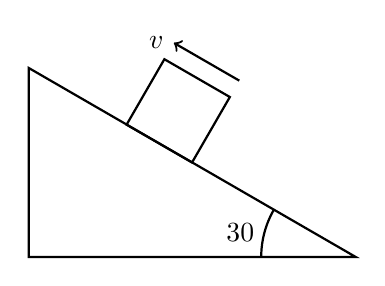
\begin{tikzpicture}[scale=1.2]
      \begin{scope}[thick]
        \draw(0,0)--(-3.46,0)--(-3.46,2)--cycle;
        \draw[thick](-1,0) arc(180:150:1) node[midway,left]{\ang{30}};
        \begin{scope}[rotate=-30]
          \draw(-2,0) rectangle(-2.8,.8);
          \draw[->](-2,1)--(-2.8,1)node[left]{$v$};
        \end{scope}
      \end{scope}
    \end{tikzpicture}
  \end{center}
  \begin{enumerate}[resume,leftmargin=18pt]
  \item Which of the following free body diagrams best represents the forces
    acting on the block as it slides up the plane?
    \begin{enumerate}[nosep,leftmargin=18pt,label=(\Alph*)]
    \item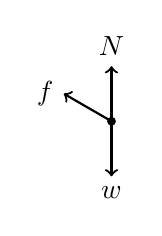
\begin{tikzpicture}[scale=.7]
      \fill[black](0,0) circle(.08);
      \draw[thick,->](0,0)--(0,1) node[above]{$\mb{N}$};
      \draw[thick,->](0,0)--(0,-1)node[below]{$\mb{w}$};
      \draw[thick,->,rotate=60](0,0)--(0,1)node[left]{$\mb{f}$};
    \end{tikzpicture}
    \item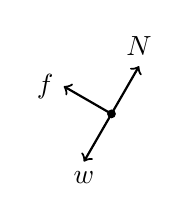
\begin{tikzpicture}[scale=.7]
        \fill[black](0,0) circle(.08);
        \draw[thick,->,rotate=-30](0,0)--(0,1)node[above]{$\mb{N}$};
        \draw[thick,->,rotate=-30](0,0)--(0,-1)node[below]{$\mb{w}$};
        \draw[thick,->,rotate=60](0,0)--(0,1)node[left]{$\mb{f}$};
    \end{tikzpicture}
    \item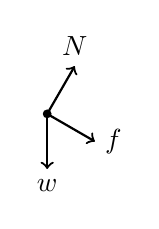
\begin{tikzpicture}[scale=.7]
      \fill[black](0,0) circle(.08);
      \draw[thick,->,rotate=-30](0,0)--(0,1)node[above]{$\mb{N}$};
      \draw[thick,->](0,0)--(0,-1)node[below]{$\mb{w}$};
      \draw[thick,->,rotate=60](0,0)--(0,-1)node[right]{$\mb{f}$};
    \end{tikzpicture}
    \item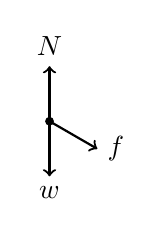
\begin{tikzpicture}[scale=.7]
      \fill[black](0,0) circle(.08);
      \draw[thick,->](0,0)--(0,1)node[above]{$\mb{N}$};
      \draw[thick,->](0,0)--(0,-1)node[below]{$\mb{w}$};
      \draw[thick,->,rotate=60](0,0)--(0,-1)node[right]{$\mb{f}$};
    \end{tikzpicture}
    \item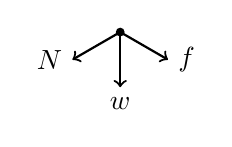
\begin{tikzpicture}[scale=.7]
      \fill[black](0,0) circle(.08);
      \draw[thick,->,rotate=120](0,0)--(0,1)node[left]{$\mb{N}$};
      \draw[thick,->](0,0)--(0,-1)node[below]{$\mb{w}$};
      \draw[thick,->,rotate=60](0,0)--(0,-1)node[right]{$\mb{f}$};
    \end{tikzpicture}
    \end{enumerate}
    \label{fbds}
    
  \item The magnitude of the frictional force $f$ between the block and the
    plane is most nearly
    \begin{enumerate}[nosep,leftmargin=18pt,label=(\Alph*)]
    \item\SI1{\newton}
    \item\SI2{\newton}
    \item\SI3{\newton}
    \item\SI4{\newton}
    \item\SI5{\newton}
    \end{enumerate}
    \label{fk}
    
%  \item A force gives an \SI{8}{\kilo\gram} mass an acceleration of
%    \SI{3}{m/s^2}. The same force will give a \SI{12}{\kilo\gram} mass an
%    acceleration of
%    \begin{enumerate}[noitemsep,topsep=0pt,leftmargin=18pt,label=(\Alph*)]
%    \item\SI{1}{\metre\per\second^2}
%    \item\SI{2}{\metre\per\second^2}
%    \item\SI{3}{\metre\per\second^2}
%    \item\SI{4}{\metre\per\second^2}
%    \item\SI{6}{\metre\per\second^2}
%    \end{enumerate}

%  \item A block weighing \SI{60}{\newton} hangs from three ropes as shown.
%    Which of the following statements is true?
%    \begin{center}
%      \vspace{-.1in}\pic{.3}{hanging}
%    \end{center}
%    \begin{enumerate}[noitemsep,topsep=0pt,leftmargin=18pt,label=(\Alph*)]    
%    \item Each rope has a tension of \SI{60}{\newton}.
%    \item The tension in each rope is higher in the lower part than in the
%      upper part of the rope.
%    \item The tension in each rope is higher in the upper part than in the
%      lower part of the rope.
%    \item The rope in the center has a higher tension than the othertwo ropes.
%    \item Each rope has a tension of \SI{20}{\newton}.
%    \end{enumerate}
    
  \item A block of mass $4m$ can move without friction on a horizontal surface.
    Another block of mass $m$ is attached to the larger block by a string that
    is passed over a light pulley. The acceleration of the system is

    \vspace{-.1in}\cpic{.25}{atwood1}
    \begin{enumerate}[nosep,leftmargin=18pt,label=(\Alph*)]
    \item $g/5$
    \item $g/2$
    \item $2g/3$
    \item $g$
    \item $5g$
    \end{enumerate}

%  \item The block of mass $4m$ in the previous question now moves on a rough
%    surface. The frictional force between the surface and the larger block is
%    equal to $\frac{1}{2}mg$. The acceleration of the system is now
%    \begin{enumerate}[noitemsep,topsep=0pt,leftmargin=18pt,label=(\Alph*)]
%    \item $\displaystyle\frac{1}{16}g$
%    \item $\displaystyle\frac{1}{10}g$
%    \item $\displaystyle\frac{1}{4}g$
%    \item $\displaystyle\frac{1}{2}g$
%    \item $g$
    %    \end{enumerate}
    \columnbreak
    
  \item Three strings are attached to a ring in the center of a force table. The
    top view of the force table is shown. For the ring to remain in the
    center of the table, which of the following must be true?
    \begin{center}
      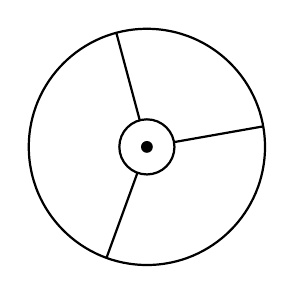
\begin{tikzpicture}[scale=.5]
        \begin{scope}[thick]
          \draw(0,0) circle(.7);
          \draw(0,0) circle(3);
          \fill(0,0) circle(.15);
          \draw[rotate=10](.7,0)--(3,0);
          \draw[rotate=105](.7,0)--(3,0);
          \draw[rotate=250](.7,0)--(3,0);
        \end{scope}
      \end{tikzpicture}
    \end{center}
    \begin{enumerate}[nosep,leftmargin=18pt,label=(\Alph*)]
    \item The vector sum of the three forces must equal zero.
    \item The lengths of the strings must be equal.
    \item The strings must form an angle of \ang{90} relative to each other.
    \item The magnitudes of two of the tensions in the strings must equal the
      tension in the third string.
    \item The tension in each string must be equal to each other.
    \end{enumerate}  
  \end{enumerate}
  
  \textbf{Questions \ref{plane1}--\ref{plane2}}

  A \SI{10}{\newton} block sits atop an inclined plane in the shape of a
  right triangle of sides \SI{3}{\metre}, \SI{4}{\metre}, and \SI{5}{\metre},
  as shown. The block is allowed to slide down the plane with negligible
  friction.
  \begin{center}
    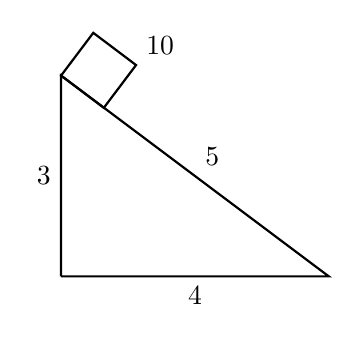
\begin{tikzpicture}[scale=.85]
      \begin{scope}[thick]
        \draw(0,0)--(4,0) node[midway,below]{\SI{4}{\metre}}
        --(0,3) node[midway,above right]{\SI{5}{\metre}}
        --(0,0) node[midway,left]{\SI{3}{\metre}};
        \draw[rotate around={-37:(0,3)}](0,3) rectangle(.8,3.8)
        node[above right]{\SI{10}{\newton}};
      \end{scope}
    \end{tikzpicture}
  \end{center}
  
  \begin{enumerate}[resume,leftmargin=18pt]
  \item The acceleration of the block is most nearly
    \begin{enumerate}[nosep,leftmargin=18pt,label=(\Alph*)]
    \item\SI2{\metre\per\second\squared}
    \item\SI4{\metre\per\second\squared}
    \item\SI6{\metre\per\second\squared}
    \item\SI{10}{\metre\per\second\squared}
    \item\SI{12}{\metre\per\second\squared}
    \end{enumerate}
    \label{plane1}
    
  \item The normal force exerted on the block by the plane is most nearly
    \begin{enumerate}[nosep,leftmargin=18pt,label=(\Alph*)]
    \item\SI{2}{\newton}
    \item\SI{4}{\newton}
    \item\SI{6}{\newton}
    \item\SI{8}{\newton}
    \item\SI{10}{\newton}
    \end{enumerate}
    \label{plane2}
  \end{enumerate}
  
  \textbf{Questions \ref{pos1}--\ref{pos2}}

  The position of a 2-kg object is described by the equation
  $x=2t^2-3t^3$, where $x$ is in meters and $t$ is in seconds.
  \begin{enumerate}[resume,leftmargin=18pt]
  \item The net force acting on the object at a time of \SI{1}{s} is
    \begin{enumerate}[nosep,leftmargin=18pt,label=(\Alph*)]
    \item\SI{-4}{\newton}
    \item\SI{-8}{\newton}
    \item\SI{-14}{\newton}
    \item\SI{-20}{\newton}
    \item\SI{-24}{\newton}
    \end{enumerate}
    \label{pos1}
    
  \item The net force acting on the object is positive from $t=0$ until a time
    of
    \begin{enumerate}[nosep,leftmargin=18pt,label=(\Alph*)]
    \item\SI{.11}{\second}
    \item\SI{.22}{\second}
    \item\SI{.44}{\second}
    \item\SI{.67}{\second}
    \item\SI{1.}{\second}
    \end{enumerate}
    \label{pos2}
%  \textbf{Questions 35-36}
%  
%  A particle of mass \SI{.5}{\kilo\gram} moves in two dimensions
%  according to the velocity equation
%  $\mb{v}=4t^2\bm{\hat{\imath}} + 6t^4 \bm{\hat{\jmath}}$, where speed is in
%  \si{m/s} and time is in \si{\second}.
%
%  \begin{enumerate}[resume,leftmargin=18pt]
%  \item The acceleration of the particle at time $t=\SI{1}{s}$ in \si{m/s^2} is
%    \begin{enumerate}[noitemsep,topsep=0pt,leftmargin=18pt,label=(\Alph*)]
%    \item $a=8\bm{\hat{\imath}} + 24\bm{\hat{\jmath}}$
%    \item $a=24\bm{\hat{\imath}} + 8\bm{\hat{\jmath}}$
%    \item $a=8\bm{\hat{\imath}} + 48\bm{\hat{\jmath}}$
%    \item $a=4\bm{\hat{\imath}} + 6\bm{\hat{\jmath}}$
%    \item $a=2\bm{\hat{\imath}} + 8\bm{\hat{\jmath}}$
%    \end{enumerate}
%
%  \item The magnitude of the net force acting on the particle at a time of
%    \SI{2}{s} is most nearly
%    \begin{enumerate}[noitemsep,topsep=0pt,leftmargin=18pt,label=(\Alph*)]
%    \item\SI{36}{\newton}
%    \item\SI{64}{\newton}
%    \item\SI{72}{\newton}
%    \item\SI{84}{\newton}
%    \item\SI{104}{\newton}
%    \end{enumerate}
   
  \item A constant force acts on a particle in such a way that the direction of
    the force is always perpendicular to its velocity. Which of the
    following is true of the particle's motion?
    \begin{enumerate}[nosep,leftmargin=18pt,label=(\Alph*)]
    \item The acceleration of the particle is increasing
    \item The acceleration of the particle is decreasing.
    \item The speed of the particle is increasing.
    \item The speed of the particle is constant.
    \item The speed of the particle is decreasing.
    \end{enumerate}
    \vspace{.7in}
    
  %\item A coffee filter is released from rest at a height of $3$ meters above
  %  the floor. Which of the following graphs best describes the speed of the
  %  falling coffee filter as a function of time?
  %  \begin{enumerate}[noitemsep,topsep=0pt,leftmargin=18pt,label=(\Alph*)]
  %  \item
  %  \item
  %  \item
  %  \item
  %  \item
  %  \end{enumerate}
  \end{enumerate}
  
  \textbf{Questions \ref{stacked1}--\ref{stacked2}}

  A block of mass \SI{2}{\kilo\gram} rests on top of a larger block of mass
  \SI{4}{\kilo\gram}. The larger block slides without friction on a table, but
  the surface between the two blocks is not frictionless. The coefficient of
  friction between the two blocks is $0.2$. A horizontal force $\mb{F}$ is
  applied to the \SI{4}{\kilo\gram} mass.
  \begin{center}
      \begin{tikzpicture}[scale=.95]
        \fill[pattern=north east lines] (3,0) rectangle(9,-.3);
        \draw[thick] (3,0)--(9,0);
        \draw[thick](5,1) rectangle(6,2) node[midway]{\SI2{\kilo\gram}};
        \draw[thick](4,0) rectangle(7,1) node[midway]{\SI4{\kilo\gram}};
        \draw[thick,->](7,.5)--(8,.5) node[right]{$\mb{F}$};
      \end{tikzpicture}
    \end{center}
  \begin{enumerate}[resume,leftmargin=18pt]
  \item What is the maximum force that can be applied such that there is no
    relative motion between the two blocks?
    \begin{enumerate}[noitemsep,topsep=0pt,leftmargin=18pt,label=(\Alph*)]
    \item zero
    \item \SI{1}{\newton}
    \item \SI{2}{\newton}
    \item \SI{4}{\newton}
    \item \SI{12}{\newton}
    \end{enumerate}
    \label{stacked1}
    
  \item What is the acceleration of the 2-kg block relative to the 4-kg block
    if a force is applied to the 4-kg block that causes the \SI4{\kilo\gram}
    block to accelerate at \SI3{\metre\per\second\squared} to the right?
    \begin{enumerate}[nosep,leftmargin=18pt,label=(\Alph*)]
    \item\SI1{\metre\per\second\squared} to the right
    \item\SI1{\metre\per\second\squared} to the left
    \item\SI2{\metre\per\second\squared} to the right
    \item\SI2{\metre\per\second\squared} to the left
    \item zero
    \end{enumerate}
    \label{stacked2}
  \end{enumerate}
\end{multicols*}

\newpage
%\begin{center}
%  {\Large
%    \textbf{AP\textsuperscript{\textregistered} Physics 1 \& C: Dynamics\\
%      Student Answer Sheet for Multiple-Choice Section}
%  }
%  
%  \begin{minipage}[t]{.3\textwidth}
%    \vspace{.2in}
%    \bgroup
%    \begin{tabular}{>{\centering}m{1.3cm} >{\centering}m{1.7cm}}
%      No. & Answer
%    \end{tabular}\\
%    \def\arraystretch{1.5}
%    \begin{tabular}{|>{\centering}m{1.3cm}|>{\centering}m{1.7cm}|}
%      \hline
%      1 & \\ \hline
%      2 & \\ \hline
%      3 & \\ \hline
%      4 & \\ \hline
%      5 & \\ \hline
%      6 & \\ \hline
%      7 & \\ \hline
%      8 & \\ \hline
%      9 & \\ \hline
%      10 & \\ \hline
%      11 & \\ \hline
%      12 & \\ \hline
%      13 & \\ \hline
%      14 & \\ \hline
%      15 & \\ \hline
%      16 & \\ \hline
%      17 & \\ \hline
%      18 & \\ \hline
%      19 & \\ \hline
%      20 & \\ \hline
%      21 & \\ \hline
%      22 & \\ \hline
%      23 & \\ \hline
%      24 & \\ \hline
%      25 & \\ \hline
%    \end{tabular}
%    \egroup
%  \end{minipage}
%    \begin{minipage}[t]{.3\textwidth}
%    \vspace{.2in}
%    \bgroup
%    \begin{tabular}{>{\centering}m{1.3cm} >{\centering}m{1.7cm}}
%      No. & Answer
%    \end{tabular}\\
%    \def\arraystretch{1.5}
%    \begin{tabular}{|>{\centering}m{1.3cm}|>{\centering}m{1.7cm}|}
%      \hline
%      26 & \\ \hline
%      27 & \\ \hline
%      28 & \\ \hline
%      29 & \\ \hline
%      30 & \\ \hline
%      31 & \\ \hline
%      32 & \\ \hline
%      33 & \\ \hline
%      34 & \\ \hline
%      35 & \\ \hline
%      36 & \\ \hline
%      37 & \\ \hline
%      38 & \\ \hline
%      39 & \\ \hline
%    \end{tabular}
%    \egroup
%  \end{minipage}
%\end{center}
%\newpage

\genfreetitle{C}{DYNAMICS}{5}

\genfreedirections

\begin{enumerate}
\item A block with mass $m$ sits on a block of mass $M$ that is resting on a
  frictionless table, as shown below. The coefficient of friction between the
  blocks are $\mu_s=0.30$ and $\mu_k=0.20$.
  \begin{enumerate}[nosep]
  \item What is the maximum force $\mb{F}$ that can be applied if the block on
    the top is not to slide on the block on the bottom.
  \item If $\mb{F}$ is half this value, find the acceleration of each block and
    the force of friction acting on each block.
  \item If $\mb{F}$ is twice the value found in (a), find the acceleration of
    each block.
  \end{enumerate}
  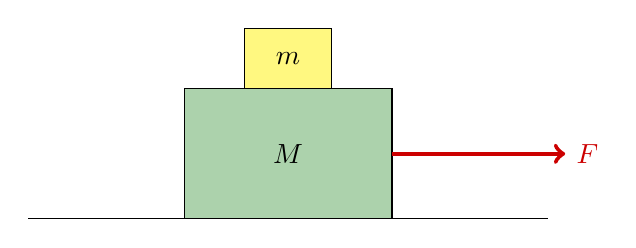
\begin{tikzpicture}[scale=1.1]
    \draw (0,0)--(6,0);
    \draw[fill=green!30!gray!50]
    (1.8,0)rectangle(4.2,1.5) node[midway,black]{$M$};
    \draw[fill=yellow!50](2.5,1.5)rectangle(3.5,2.2)
    node[midway,black]{$m$};
    \draw[ultra thick,red!80!black,->](4.2,.75)--(6.2,.75)
    node[right]{$\mb{F}$};
  \end{tikzpicture}
  \vspace{2.25in}
  \newpage
  
\item A \SI{2.}{\kilo\gram} body rests on a smooth wedge that has an inclination
  of \ang{60} and an acceleration $\mb{a}$ to the right such that the mass
  remains stationary relative to the wedge.
  \begin{enumerate}
  \item Find acceleration $\mb{a}$.
  \item What would happen if the wedge were given a greater acceleration?
  \end{enumerate}
  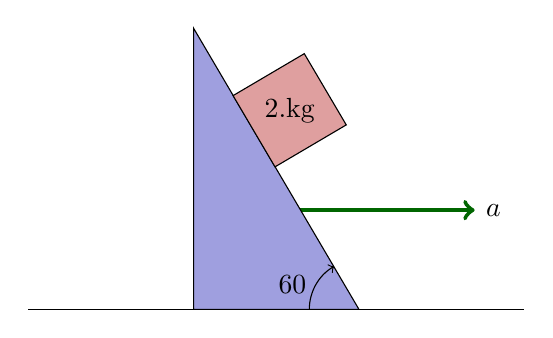
\begin{tikzpicture}[scale=2.1]
    \draw[ultra thick,green!40!black,->](.5,.6)--(1.7,.6)
    node[right,black]{$\mb{a}$};
    \draw(-1,0)--(2,0);
    \draw[fill=blue!50!gray!50](0,0)--(0,1.7)--(1,0)--cycle;
    \draw[->](.7,0) arc(180:120:.3) node[midway,left]{\ang{60}};
    \begin{scope}[rotate around={-59.5:(1,0)}]
      \draw[fill=red!50!gray!50](0,0) rectangle(-.5,.5)
      node[midway,black]{\SI{2.}{kg}};
    \end{scope}
  \end{tikzpicture}
  \newpage
  
\item A pick-up truck with two stacked crates in the truck bed brakes quickly.
  The crate on the bottom just barely stays put on the bed of the truck. Does
  the top crate stay put or does it fall off? The top crate has a mass of
  \SI{27}{\kilo\gram} and the mass of the bottom crate is \SI{22}{\kilo\gram}.
  The coefficient of static friction between the bottom crate and the truck is
  $0.42$, and the coefficient of kinetic friction for that surface is $0.35$.
  The coefficient of static friction between the crate is $0.40$, and the
  coefficient of kinetic friction is $0.32$.
  \vspace{2in}
  \newpage

%  % THIS QUESTION IS TO BE REMOVED AFTER SUMMER 2020 SESSION
%\item A bucket with mass $m_2$ and a block with mass $m_1$ are hung on a pulley
%  system. Find the magnitude of the acceleration with which the bucket and the
%  block are moving and the magnitude of the tension force $T$ by which the rope
%  is stressed. Ignore the masses of the pulley system and the rope. The bucket
%  moves up and the block moves down.
%  \begin{center}
%    \pic{.18}{pulley-system}
%  \end{center}
%  \newpage

  % THIS IS TAKEN FROM THE 2013 AP PHYSICS C FREE-RESPONSE QUESTION MECH 2
  \begin{center}
    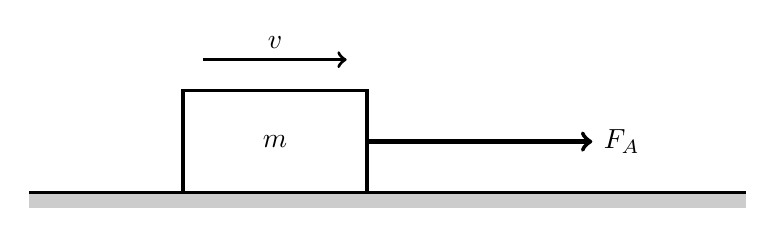
\begin{tikzpicture}[scale=1.3]
      \fill[gray!40](-1.5,-.15) rectangle(5.5,0);
      \begin{scope}[very thick]
        \draw(-1.5,0)--(5.5,0);
        \draw(0,0) rectangle(1.8,1) node[midway]{$m$};
        \draw[->](.2,1.3)--(1.6,1.3) node[midway,above]{$v$};
      \end{scope}
      \draw[ultra thick,->](1.8,.5)--(4,.5) node[right]{$F_A$};
    \end{tikzpicture}
  \end{center}
\item A box of mass $m$ initially at rest is acted upon by a constant applied
  force of magnitude $F_A$, as shown in the figure above. The friction between
  the box and the horizontal surface can be assumed to be negligible, but the
  box is subject to a drag force of magnitude k u where u is the speed of the
  box and k is a positive constant. Express all your answers in terms of the
  given quantities and fundamental constants, as appropriate.
  \begin{enumerate}[leftmargin=15pt]
  \item The dot below represents the box. Draw and label the forces (not
    components) that act on the box.
    \vspace{.5in}
    \begin{center}
      {\tikz\fill(0,0) circle(.2);}
    \end{center}
    \vspace{.5in}

  \item Write, but do not solve, a differential equation that could be used to
    determine the speed $v$ of the box as a function of time $t$. If you need
    to draw anything other than what you have shown in part (a) to assist in
    your solution, use the space below. Do NOT add anything to the figure in
    part (a).
    \vspace{1.25in}
  \item Determine the magnitude of the terminal velocity of the box.
    \vspace{1.25in}
  \item Use the differential equation from part (b) to derive the equation for
    the speed $v$ of the box as a function of time $t$. Assume that $v=0$ at
    time $t=0$.
    \vspace{1.25in}
    \newpage
    
  \item On the axes below, sketch a graph of the speed $v$ of the box as a
    function of time $t$. Explicitly label any intercepts, asymptotes, maxima,
    or minima with numerical values or algebraic expressions, as appropriate.
    \begin{center}
      \begin{tikzpicture}
        \draw[very thick,->](0,0)--(4,0)
        node[pos=0,left]{$O$} node[right]{$t$};
        \draw[very thick,->](0,-3)--(0,3)node[above]{$v$};
      \end{tikzpicture}
    \end{center}
  \end{enumerate}
  \vspace{.3in}
  \newpage
  
  % THIS IS TAKEN FROM THE 2011 AP PHYSICS C FREE-RESPONSE QUESTION MECH 2
  \begin{center}
    \pic{.5}{amusement}
  \end{center}
\item An amusement park ride features a passenger compartment of mass $M$ that
  is released from rest at point $A$, as shown in the figure above, and moves
  along a track to point $E$. The compartment is in free fall between points $A$
  and $B$, which are a distance of $3R/4$ apart, then moves along the circular
  arc of radius $R$ between points $B$ and $D$. Assume the track is
  frictionless from point $A$ to point $D$ and the dimensions of the passenger
  compartment are negligible compared to $R$.
  \begin{enumerate}[leftmargin=15pt]
  \item  On the dot below that represents the passenger compartment, draw and
    label the forces (not components) that act on the passenger compartment
    when it is at point $C$, which is at an angle $\theta$ from point $B$.
    \begin{center}
      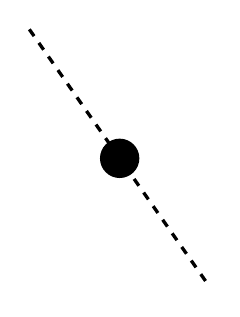
\begin{tikzpicture}
        \fill(0,0) circle(.25);
        \draw[rotate=35,dashed,very thick](0,2)--(0,-2);
      \end{tikzpicture}
    \end{center}
    
  \item In terms of $\theta$ and the magnitudes of the forces drawn in part
    (a), determine an expression for the magnitude of the centripetal force
    acting on the compartment at point $C$. If you need to draw anything
    besides what you have shown in part (a) to assist in your solution, use the
    space below. Do NOT add anything to the figure in part (a).
    \vspace{\stretch1}
    
  \item Derive an expression for the speed $v_D$ of the passenger compartment
    as it reaches point $D$ in terms of $M$, $R$, and fundamental constants, as
    appropriate.
    \vspace{\stretch1}
  \end{enumerate}
  \newpage
  A force acts on the compartment between points $D$ and $E$ and brings it to
  rest at point $E$.
  \begin{enumerate}[resume]
  \item If the compartment is brought to rest by friction, calculate the
    numerical value of the coefficient of friction $\mu$ between the
    compartment and the track.
    \vspace{1in}
  \item Now consider the case in which there is no friction between the
    compartment and the track, but instead the compartment is brought to rest
    by a braking force $-k\mb{v}$, where $k$ is a constant and $\mb{}$v is the
    velocity of the compartment. Express all algebraic answers to the following
    in terms of $M$, $R$, $k$, $v_D$, and fundamental constants, as
    appropriate.
    \begin{enumerate}
    \item Write, but do NOT solve, the differential equation for $v(t)$.
      \vspace{\stretch1}
    \item Solve the differential equation you wrote in part i.
      \vspace{\stretch1}
    \item On the axes below, sketch a graph of the magnitude of the
      acceleration of the compartment as a function of time. On the axes,
      explicitly label any intercepts, asymptotes, maxima, or minima with
      numerical values or algebraic expressions, as appropriate.
      \begin{center}
        \begin{tikzpicture}
        \draw[very thick,->](0,0)--(7,0) node[midway,below]{Time};
        \draw[very thick,->](0,0)--(0,3) node[above]
             {Magnitude of Acceleration};
        \end{tikzpicture}
      \end{center}
    \end{enumerate}
  \end{enumerate}
\end{enumerate}

\end{document}
